\documentclass[../SimBALink.tex]{subfiles}
\begin{document}

This system models the gear and chain in such a way to allow for wheel slip. 

\subsection{Inputs and outputs}
	\paragraph{Inputs}
	\begin{tabular}{ l | l | l  }
		Input					&	Symbol		&	Unit		\\	\hline
		Motor Torque			& 	$\tau_m$ 		& Nm \\
		Tire Torque				&	$\tau_t$	&	Nm
	\end{tabular}
	
	\paragraph{Outputs}
	\begin{tabular}{ l | l | l  }
		Output					&	Symbol		&	Unit		\\	\hline
		Tire Velocity		&	$\omega_t$		&	rad/s \\
		Gear Torque			&	$\tau_g$		& Nm
	\end{tabular}

\subsection{Background, rationale, modeling strategy}
The tire, chain, gear, and motor are modeled as a lumped inertia that is accelerated by the motor torque and tire torque(modeled as a load). The chain is modeled lossey through an efficiency map. Gearing is modeled as a ratio that linearly changes motor torque to gear torque. This method of modeling allows for wheel slip down the line.
		\begin{gather}
		\dot{\omega_t} = \frac{\tau_g - \tau_t}{J_m + J_g + J_t + J_c} \\
		\tau_g = \frac{\tau_m \eta_c (\omega_t)}{R_g}
		\end{gather}

\subsection{States}
	\begin{tabular}{ l | l | l  }
		State					&	Symbol		&	Unit		\\	\hline
		Tire Velocity 			&	$\omega_t$	&	rad/s
	\end{tabular}

\subsection{Parameters}
	\begin{tabular}{ l | l | l  }
		Parameters					&	Symbol		&	Unit		\\	\hline
		Motor inertia		&	$J_m$		&	 $kg*m^2$ \\ 
		Gear inertia		&	$J_g$		&	 $kg*m^2$ \\ 
		Chain inertia		&	$J_c$		&	 $kg*m^2$ \\ 
		Tire inertia		&	$J_t$		&	 $kg*m^2$ \\ 
		Gear Ratio			&	$R_g$		&	$\frac{\tau_g}{\tau_m}$
	\end{tabular}
	
\subsection{Functions}
$\eta_c(\omega_t)$ \\
	\begin{tabular}{ l | l | l | l }
		Type				& Description		&	Symbol		&	Unit		\\	\hline
		Input 				& Wheel Speed		&	$\omega_t$  & 	rad/s		\\
		Output 				& Chain Efficiency	&	n/a			&	\%
	\end{tabular} \\

The function is modeled as a look up table following the curve below described in the paper "Optimization of Chain Drives in Sports Motorcycles".

\begin{figure}[h!]
  \centering
  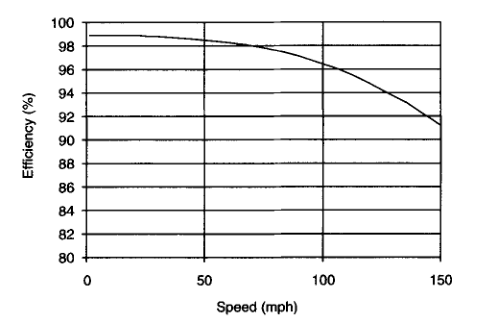
\includegraphics[scale=1]{Chain_Efficiency}
  \caption{Estimated Chain Efficiency}
\end{figure}

\subsection{Assumptions}
\begin{itemize}
  \item The chain and gearing is rigid (no chain/gear dynamics)
  \item Chain efficiency is only a function of wheel speed
\end{itemize}

\subsection{Validation}

The model was subjected to a motor torque of 10 and an increasing tire torque. The model works correctly. The wheel increases in speed and the correctly models the losses in the chain.


\begin{figure}[H]
\center
  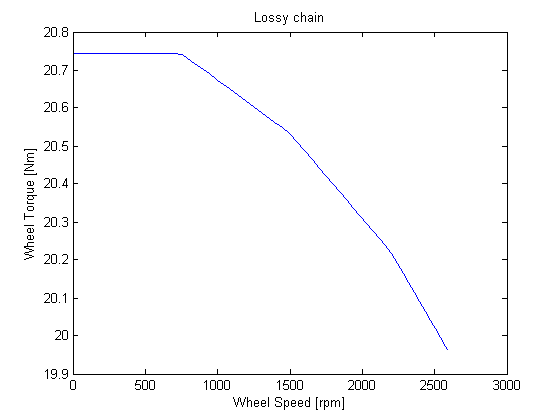
\includegraphics[scale=.5]{gear_val_lossy_chain}
  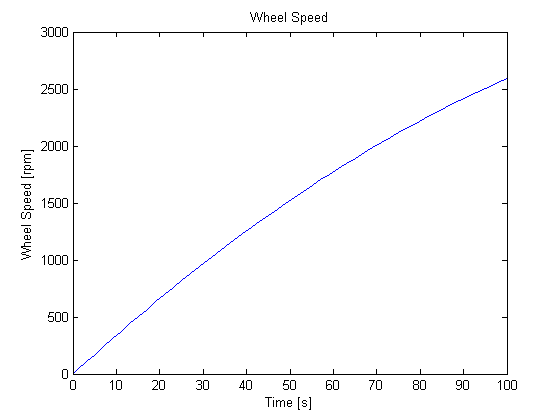
\includegraphics[scale=.5]{gear_val_spin_up}
  \caption{Gear and Chain Validation}
\end{figure}







\end{document}